\documentclass[12pt]{article}

\usepackage[utf8]{inputenc}
\usepackage[portuguese]{babel}
\usepackage{amsmath,bm,bbm} 
\usepackage{booktabs}
\usepackage{graphicx}
\usepackage{etoolbox}
\usepackage{url}     
\usepackage{changepage}
\usepackage{titlesec}
\usepackage{hyperref}
\usepackage[parfill]{parskip}
\usepackage[margin=1in]{geometry}
\usepackage{times}
\usepackage{cite}
\usepackage{tabularx}
\usepackage{lipsum} 
\usepackage{graphicx}
\titleformat*{\section}{\normalsize\bfseries}
\font\myfont=cmr10 at 10pt

%----------------------------------------------------------------------------------------
%  Título do trabalho
%----------------------------------------------------------------------------------------
\title{\large \textbf{Um breve estudo sobre Análise não-paramétrica de Séries Temporais utilizando descritores causais oriundos da Teoria da Informação}}
 \author{\myfont Eduarda T.\ C.\ Chagas \\ \myfont Universidade Federal de Alagoas - Instituto de Computação \\  \myfont eduardachagas48@laccan.ufal.br \\
 \myfont Milena B. Nunes \\ \myfont Universidade Federal de Alagoas - Instituto de Computação \\ \myfont mbn@laccan.ufal.br \\
 \myfont Alejandro C.\ Frery \\ \myfont Universidade Federal de Alagoas - Laboratório de Computação Científica e Análise Numérica \\ \myfont acfrery@laccan.ufal.br \\}
\date{}

\makeatletter 
\patchcmd{\@maketitle}{\begin{center}}{\begin{adjustwidth}{0.5in}{0.5in}\begin{center}}{}{}
\patchcmd{\@maketitle}{\end{center}}{\end{center}\end{adjustwidth}}{}{}
\makeatother

%----------------------------------------------------------------------------------------

\begin{document}
\raggedright
\maketitle
\thispagestyle{empty}
\pagestyle{empty}

\textbf{Resumo:} Este trabalho descreve algumas das principais técnicas e ferramentas disponíveis na literatura para a análise não-paramétrica de séries temporais utilizando descritores da Teoria da Informação, focando nos conceitos e metodologias aplicados com sucesso em diversos ramos de pesquisa científica.

\textbf{Palavras-chave:} Séries Temporais, Análise não-paramétrica, Teoria da Informação, Computação Científica.

 
\section*{Introdução}

Séries temporais são conjuntos de dados adquiridos sequencialmente a partir de um processo observacional ao longo do tempo não necessariamente dividido em espaços iguais.

As séries temporais se caracterizam por exibir dependência serial entre os seus elementos.

O estudo de séries temporais auxilia na análise das propriedades de sistemas.
A sua aplicação pode ser encontrada em múltiplas áreas do conhecimento científico como, por exemplo,
a discriminação entre fenômenos estocásticos e caóticos~\cite{DistinguishingNoiseFromChaos}, 
a identificação de padrões de comportamento em redes veiculares~\cite{CharacterizationVehicleBehaviorInformationTheory}, 
a classificação e verificação de assinaturas \textit{online}~\cite{ClassificationVerificationOnlineHandwrittenSignatures},
a análise da eficiência informacional do mercado de petróleo~\cite{oilMarket},
a caracterização das séries temporais produzidas por eletroencefalogramas~\cite{EGGTimeSeries},
na análise da robustez de redes~\cite{InformationTheoryPerspectiveNetworkRobustness}, e 
a classificação de padrões de consumo de energia elétrica~\cite{CharacterizationElectricLoadInformationTheoryQuantifiers}.

O estudo de séries temporais é tradicionalmente dividido em duas linhas de estudo, nos domínios do tempo e da frequência~\cite{BrockwellDavis91}.

No entanto, ambas abordagens utilizam diretamente os dados resultantes do processo observacional, que são sensíveis a efeitos provocados por diversos tipos de contaminação.

A abordagem do uso de métodos não paramétricos surge na literatura como uma forma de evitar que tais efeitos invalidem as análises.

A Teoria da Informação, desenvolvida por Claude Shannon~\cite{shannon}, é uma ferramenta poderosa para a quantificação de sistemas dinâmicos.

Conceitos como a Entropia de Shannon auxiliam da análise de mercados~\cite{hart} até dinâmicas não-lineares~\cite{fisherRosso}.

Neste trabalho apresentamos de forma unificada o uso de descritores oriundos da Teoria da Informação na análise de séries temporais.

O trabalho está organizado como segue.
A Seção~\ref{sec:dois}, apresenta as principais representações do espaço de probabilidade de séries temporais. 
A entropia de permutação e as suas variações são apresentadas na Seção~\ref{sec:tres}. 
A Seção~\ref{sec:quatro} descreve algumas distâncias estocásticas. 
Na Seção~\ref{sec:cinco} falaremos sobre Complexidade Estatística e o Plano Entropia-Complexidade.

\section{Representação do espaço de probabilidade e a Distribuição de Bandt e Pompe}
\label{sec:dois}

A transformação de uma série temporal em uma distribuição de probabilidade (PDF) \texttt P permite avaliar o conteúdo informacional acerca da dinâmica do sistema e dos processos subjacentes, descrevendo-os de forma mensurável e observável~\cite{entropyAndInformationTheory}.
Através desta caracterização é possível utilizar de métricas do espaço PDF, permitindo comparar diferentes conjuntos e classificá-los de acordo com as propriedades dos processos subjacentes. 
Podemos assim, por exemplo, classificar uma série entre estocástica ou determinística.

A ideia das técnicas não paramétricas consiste em construir o histograma de algum atributo da série temporal, e extrair dele métricas de Teoria da Informação.
Os atributos são os mais variados~\cite{Kowalski2011DistancesIP}, dentre eles: 
(a)~padrões ordinais~\cite{ROSSO2}, 
(b)~histogramas~\cite{article3,DEMICCO20083373},
(c)~dinâmica simbólica binária~\cite{PhysRevLett}, 
(d)~Análise de Fourier~\cite{article}, e 
(e)~transformada wavelet~\cite{ROSSO3}. 
Todas estas metodologias são capazes de capturar aspectos globais de dinâmicas complexas. 

No entanto, não é trivial encontrar uma representação simbólica significativa da série original. 
A abordagem de Bandt e Pompe~\cite{article2}, por considerar a causalidade temporal dos dados, revela detalhes importantes da estrutura ordinal da série temporal.

A metodologia de Bandt e Pompe consiste em transformar a série temporal, por meio de transformação não paramétrica, em uma sequência de padrões.
Seja a série $\bm x = (x_1, x_2, \dots, x_n)$; cada grupo de $N$ valores (não necessariamente adjacentes) será transformado em um padrão ordinal, para depois formar o histograma das suas ocorrências na série.
Por exemplo, com $N=3$ e para qualquer $i$,
se $x_i<x_{i+1}<x_{i+2}$ esta tripla será associada ao padrão $\pi_0$; 
caso $x_i>x_{i+1}>x_{i+2}$ o padrão será $\pi_1$, e assim por diante.
Há $N!$ possíveis padrões.

A literatura apresenta duas maneiras de definir o mapeamento de padrões:  
(a)~ordenando as posições dos grupos em ordem cronológica (Permutação de Classificação), e 
(b)~ordenando os índices de tempo de acordo fileiras dos elementos do subconjunto (Permutação do Índice Cronológico)~\cite{tiedvalues}.

Uma vez calculado o histograma de padrões $\bm h=(h_1,\dots,h_{N!})$, o próximo passo é obter descritores.

\section{Entropia de permutação}
\label{sec:tres}

A Entropia mede o desordem ou a imprevisibilidade de um sistema caracterizado por uma função de probabilidade $\bm h$.
Neste trabalho citaremos três modelos de entropia: de Shannon, de Tsallis e de R\'enyi.

Proposta em 1948, a entropia de Shannon consiste de uma variação da Entropia de Boltzmann-Gibbs~\cite{shannon}.
Ela é definida por $H(\bm h) = -\sum_{i}^{n} h_i \log h_i $, com a convenção $-0\infty=0$.
Os seus valores mínimo ($0$) e máximo ($1!$) ocorrem para os casos em que um único evento tem probabilidade $1$, e para eventos equiprováveis, respectivamente, isto é, para a certeza e a incerteza completas. 

Tsallis propôs um novo modelo~\cite{entropyInformation}, ampliando o  conjunto de aplicações abordado por Boltzmann:
$H_a(\bm h) ={(a-1)}^{-1}(1 - \log \sum_{i=1}^{N!}h_i^a)$, com $a \neq 1$.

A entropia de R\'enyi é uma generalização da entropia de Shannon, sendo aplicada em Teoria da Informação como um índice estatístico de diversidade ou aleatoriedade~\cite{Tsallis1988}: $H_a(\bm h) ={(1-a)^{-1}}\log \sum_{i=1}^{N!}h_i^a$.


\section{Distância Estocástica}
\label{sec:quatro}

A habilidade da Entropia capturar propriedades do sistema é limitada.
Outras medidas interessantes são distâncias entre o histograma de padrões $\bm h$ e uma medida de probabilidade que descreva um processo não informativo, tipicamente a distribuição uniforme.
A Tabela~\ref{Tab:Distancias} mostra algumas possíveis medidas de distância $d(\bm p,\bm q)$ entre duas funções de probabilidade $\bm p=(p_1,\dots)$ e $\bm q=(q_1,\dots)$, definidas sobre o mesmo suporte.

\begin{table}[hbt]
\caption{Distâncias Estocásticas}\label{Tab:Distancias}
\centering
\begin{tabular}{lc}\toprule
Euclidiana					& $ \sqrt{\sum_i(q_i-p_i)^{2}}$\\
Manhattan					& $ \sum_{i}|q_i-p_i|$\\
Chebyshev					& $ \max_i\{|q_i-p_i|\}$\\
Kullback-Leibler			& $ \sum_{i}q_i \log\frac{q_i}{p_i}$\\
Jensen-Shannon				& $ \sum_{i} \Big(p_i \log\frac{p_i}{q_i} + q_i \log\frac{q_i}{p_i}\Big)$\\
Wotters						& $ \cos^{-1}\sum_{i} \sqrt{p_i q_i}$ \\
Bhattacharya				& $ -\log\sum_{i}\sqrt{p_i q_i}$ \\
\bottomrule
\end{tabular}
\end{table}

Outras distâncias e relações entre elas podem ser vistas no livro de Deza e Deza~\cite{EncyclopediaofDistances}.

\section{Complexidade Estatística e o Plano HC}
\label{sec:cinco}

Uma Entropia e uma Distância podem ser combinadas no atributo Complexidade Estatística: $C(\bm h, \bm p) = H(\bm h)d(\bm h, \bm p)$ para aumentar o seu poder de descrição~\cite{article5,FELDMAN1998244,LOPEZRUIZ1995321}:
Uma escolha conveniente é a complexidade de Jensen-Shannon, dada por
 \begin{equation}
 C_{\text{JS}}(\bm h) = H_{\text{S}}(\bm h) . Q_{\text{JS}}(\bm h, \bm p),
 \end{equation}
em que $H_{\text{S}}$ é a entropia de Shannon normalizada, $\bm h$ o histograma dos padrões ordinais, $\bm p$ a distribuição uniforme e $Q_{\text{JS}}$ é a distância de Jensen-Shannon.
 
Cada série temporal $\bm x$ pode, então, ser mapeada no ponto $(H_{\text{S}}, C_{\text{JS}})$.
O conjunto de todos os pontos possíveis forma o \textit{mapa Entropia-Complexidade}, e a posição do ponto nesse plano é um descritor das propriedades da dinâmica subjacente à série~\cite{OrdinalPatternProbabilities}.
A forma desse plano depende do comprimento $N$ dos padrões~\cite{MARTIN2006439}.

\begin{figure}[hbt]
		\centering
		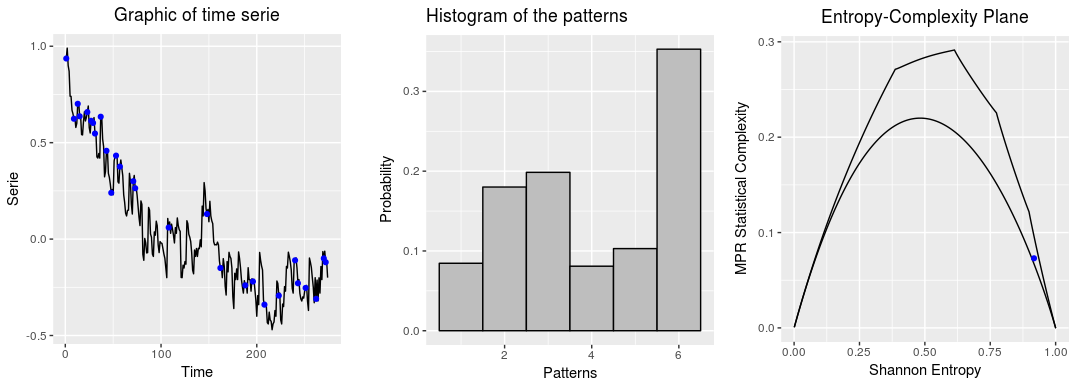
\includegraphics[width=1\columnwidth]{img1}        
	\caption{A figura acima ilustra o processo de extração de informações de uma série temporal que representa anomalias médias globais da temperatura em graus Celsius em relação a um período base (GISTEMP e GCAG).  Os dados se encontram disponíveis em \url{https://pkgstore.datahub.io/core/global-temp/annual_csv/data/a26b154688b061cdd04f1df36e4408be/annual_csv.csv}. A imagem 1.1 nos informa a presença dos padrões $(2,0,1)$ na série. Já a imagem 1.2 apresenta o histograma de densidade, utilizado posteriormente como função de probabilidade. Por último, a figura 1.3 no mostra a representação de tais dados no Plano HC}
	\label{fig:Img1}
\end{figure}


\section*{Conclusões}

Neste trabalho apresentamos de forma unificada uma revisão da literatura sobre a teoria e a aplicação da técnica de simbolização de séries temporais pelo método de Bandt e Pompe.
 

%-------------------------------------------------------------------
%  Referências bibliográficas
%-------------------------------------------------------------------
\bibliographystyle{unsrt} 
\bibliography{ref}

\end{document}